\documentclass[11pt]{article}

\newcommand{\numpy}{{\tt numpy}}    % tt font for numpy
\usepackage{amsmath,amssymb}
\usepackage[utf8]{inputenc}
\usepackage[english]{babel}
\usepackage{graphicx}
\topmargin -1.in
\textheight 10in
\oddsidemargin -.75in
\evensidemargin -.75in
\textwidth 7in

\begin{document}

% ========== Edit your name here
\author{Anthony}
\title{VXB Vectors}
\maketitle

% ========== Begin answering questions here
\begin{figure}[h]
\centering
  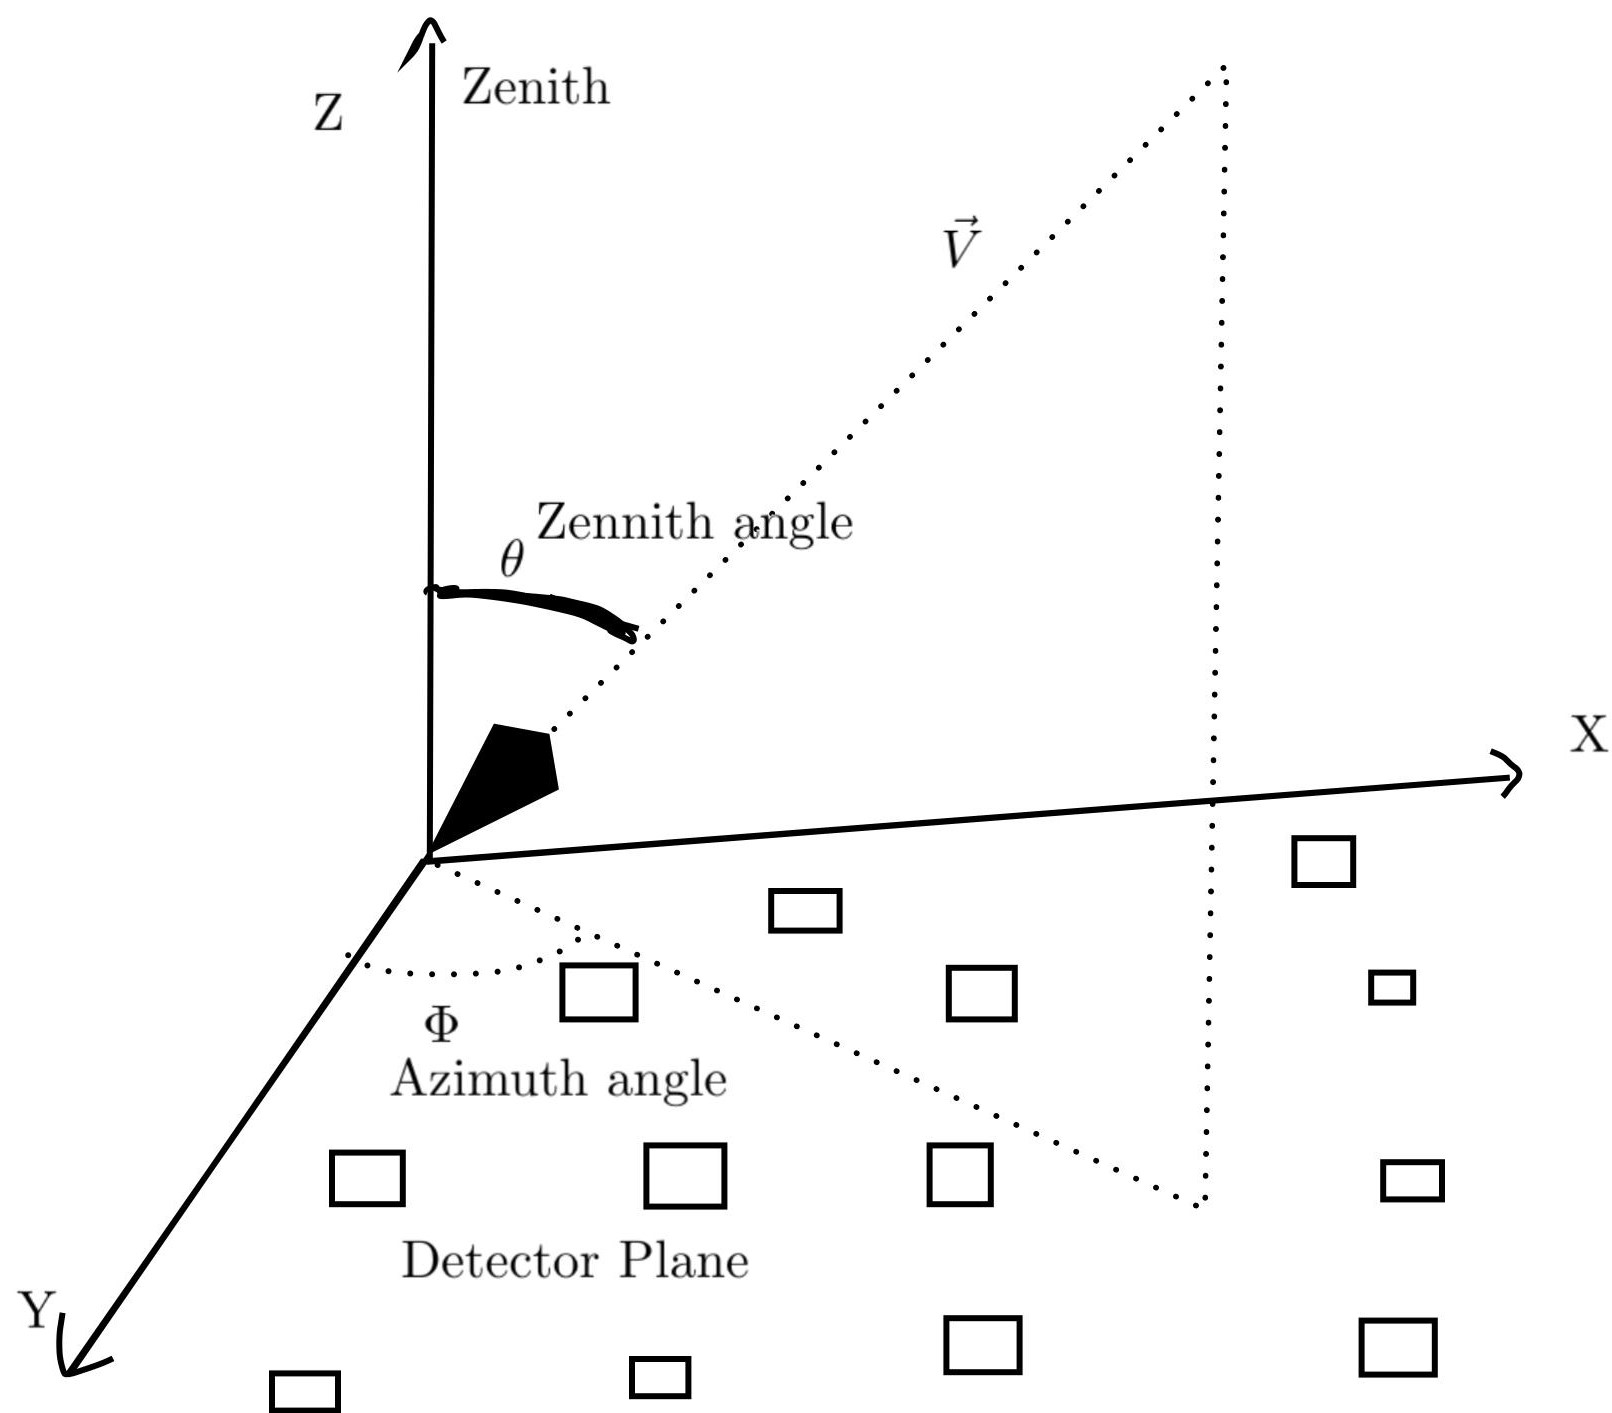
\includegraphics[scale=0.2]{vvv.JPG}
  \caption{Detector to shower plane }
  \label{fig:boat1}
\end{figure}

To start the coordinate transformation from the detector plane to the show plane, the unit vector of the velocity of the incoming shower is to be  described in the detector plane co-ordinates noting the zenith angle $\theta$ with respect to the positive z-axis and the azimuth angle $\phi$ taken with respect to the positive x-axis  . The $\mathbf{-\hat{v}}$ is then set to be the new zenith via the following transformation where $|\hat{v}|$ is the length of the velocity vector:
\begin{equation}
    \mathbf{\hat{z}'}=\mathbf{-\hat{v}} = \frac{-1}{\left|\vec{v}\right|}\left(
    \begin{array}{c}
    v\sin\theta \cos\phi \\ 	
    v\sin\theta \sin\phi \\ 
    v\cos\theta \\
\end{array} 
\right)
\end{equation}



The magnetic field unit $\mathbf{\hat{B}}$ vector can be written out explicitly as:
\begin{equation}
   \mathbf{\hat{B}}=\frac{1}{\left|\vec{B}\right|} \left(
    \begin{array}{c}
    B\sin\theta_B \\ 	
    B\sin\theta_B\\ 
    B\cos\theta_B \\
\end{array} 
\right),  \mbox{  where $\theta_B$ is the magnetic field inclination angle.}
\end{equation}

To generate a second axis that is perpendicular to both the $\mathbf{\hat{v}}$ and and magnetic field  $\mathbf{\hat{B}}$, we get the cross product of both unit vectors.

\begin{equation}
    \mathbf{\hat{x}'} =\mathbf{-\hat{v}}\times \mathbf{\hat{B}} = det \left(
    \begin{array}{ccc}
    i & j & k \\ 	
   - \sin\theta \cos\phi & -\sin\theta \sin\phi  & -\cos\theta \\ 
     \sin\theta_B& \sin\theta_B & \cos\theta_B\\
\end{array} 
\right)
\end{equation}

\begin{equation}
   \mathbf{\hat{x}'}=\left(
    \begin{array}{c}
    -\sin\theta\sin\phi\cos\theta_B + \cos\theta\sin\theta_B\\ 	
    -\cos\theta\sin\theta_B+\sin\theta\cos\phi\cos\theta_B\\ 
    -\sin\theta\cos\phi\sin\theta_B+\sin\theta\sin\phi\sin\theta_B \\
\end{array} 
\right) 
\end{equation}

The third axis is then a cross product of   $\mathbf{-\hat{v}}$ and $\mathbf{-\hat{v}}\times \mathbf{\hat{B}}$ ,this creates a 3rd mutually perpendicular axis to both $\mathbf{-\hat{v}}$ and $\mathbf{-\hat{v}}\times \mathbf{\hat{B}}$ i.e. $\mathbf{-\hat{v}} \times\mathbf{-\hat{v}}\times \mathbf{\hat{B}}$. 

\small
\begin{equation}
    \mathbf{\hat{y}'}=\mathbf{-\hat{v}}\times \mathbf{-\hat{v}\times\hat{B} } = det \left(
    \begin{array}{ccc}
    i & j & k \\ 	
   - \sin\theta \cos\phi & -\sin\theta \sin\phi  & -\cos\theta \\ 
      -\sin\theta\sin\phi\cos\theta_B + \cos\theta\sin\theta_B&  -\cos\theta\sin\theta_B+\sin\theta\cos\phi\cos\theta_B &  -\sin\theta\cos\phi\sin\theta_B+\sin\theta\sin\phi\sin\theta_B\\
\end{array} 
\right)
\end{equation}
% ========== Continue adding items as needed

\begin{equation}
   \mathbf{\hat{y}'}=\left(
    \begin{array}{c}
     (-\sin\theta \sin\phi )*(-\sin\theta\cos\phi\sin\theta_B+\sin\theta\sin\phi\sin\theta_B)-     (\cos\theta)  *(-\cos\theta\sin\theta_B+\sin\theta\cos\phi\cos\theta_B )   \\ 
(-\sin\theta \cos\phi )(-\sin\theta\cos\phi\sin\theta_B+\sin\theta\sin\phi\sin\theta_B )+(-\cos\theta)*( -\sin\theta\sin\phi\cos\theta_B + \cos\theta\sin\theta_B)\\
 
    (-\sin\theta \cos\phi )*(-\cos\theta\sin\theta_B+\sin\theta\cos\phi\cos\theta_B)-(-\sin\theta \sin\phi )*(-\sin\theta\sin\phi\cos\theta_B + \cos\theta\sin\theta_B)
\end{array} 
\right) 
\end{equation}

In an orientation that will give rise to the relationship $\mathbf{-\hat{v}} \times \left( \mathbf{-\hat{v}} \times\mathbf{-\hat{v}}\times \mathbf{\hat{B}}\right) = \mathbf{-\hat{v}}\times \mathbf{\hat{B}} $ , $\left(\mathbf{-\hat{v}}\times \mathbf{\hat{B}}\right) \times \left( \mathbf{-\hat{v}} \times\mathbf{-\hat{v}}\times \mathbf{\hat{B}}\right) = \mathbf{-\hat{v}}$ or $\hat{x}' \times \hat{y}'=\hat{z}' $ and can be tested for orthogonality via the dot product = 0 test.
\end{document}
\grid
\grid